\documentclass[tikz, border=2pt]{standalone}
\usepackage{tikz}
\usetikzlibrary{arrows.meta,positioning,fit,backgrounds,calc}
% Shared TikZ style, color-matched to paper/figures/*.pdf (matplotlib):
% ink = near-black strokes/fill, accent = deep red for the one thing per
% diagram that should draw the eye, grid = light gray for structure that
% should recede.
\definecolor{ink}{HTML}{1A1A1A}
\definecolor{accent}{HTML}{A6192E}
\definecolor{gridgray}{HTML}{D9D9D9}
\definecolor{panelbg}{HTML}{F2F2F2}

\tikzset{
  every node/.style={font=\sffamily},
  box/.style={draw=ink, thick, rounded corners=1.5pt, minimum height=0.75cm,
              font=\sffamily\small, align=center, fill=white, text=ink},
  stubbox/.style={box, draw=ink, dashed, fill=panelbg},
  hibox/.style={box, fill=ink, text=white},
  panel/.style={draw=none, fill=panelbg, rounded corners=2pt},
  arr/.style={-{Latex[length=2.2mm, width=1.6mm]}, thick, draw=ink},
  darr/.style={arr, dashed},
  accarr/.style={-{Latex[length=2.2mm, width=1.6mm]}, thick, draw=accent},
  lbl/.style={font=\sffamily\scriptsize, text=ink},
  ital/.style={font=\sffamily\itshape\scriptsize, text=ink!70},
  note/.style={font=\sffamily\scriptsize, align=left, text=ink},
  state/.style={draw=ink, thick, rounded corners=3pt, minimum width=2.6cm,
                minimum height=0.9cm, font=\sffamily\small, align=center, fill=white},
  finalstate/.style={state, fill=ink, text=white},
  abortstate/.style={state, draw=accent, thick, text=accent},
}

\begin{document}
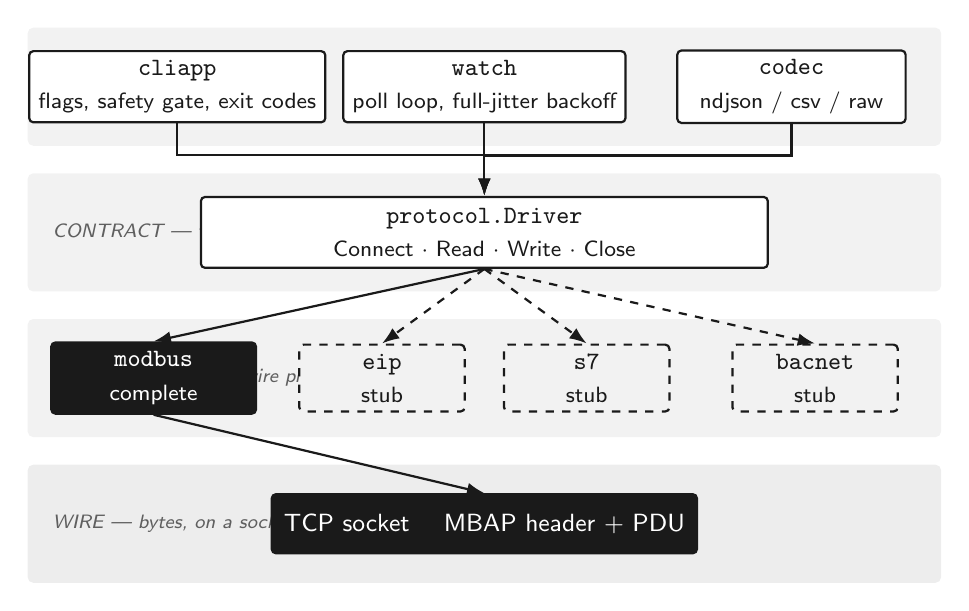
\begin{tikzpicture}[node distance=6mm]

% --- layer panels (drawn first, as background) ---
\begin{scope}[on background layer]
\node[panel, minimum width=11.6cm, minimum height=1.5cm] (p1) at (0,4) {};
\node[panel, minimum width=11.6cm, minimum height=1.5cm] (p2) at (0,2.15) {};
\node[panel, minimum width=11.6cm, minimum height=1.5cm] (p3) at (0,0.3) {};
\node[panel, minimum width=11.6cm, minimum height=1.5cm, fill=ink!8] (p4) at (0,-1.55) {};
\end{scope}

\node[ital, anchor=west] at ([xshift=2mm]p1.west) {CLI --- one flag, one job};
\node[ital, anchor=west] at ([xshift=2mm]p2.west) {CONTRACT --- the only boundary a driver may cross};
\node[ital, anchor=west] at ([xshift=2mm]p3.west) {DRIVERS --- one per wire protocol};
\node[ital, anchor=west] at ([xshift=2mm]p4.west) {WIRE --- bytes, on a socket};

% --- layer 1: cli ---
\node[box, minimum width=2.9cm] (flags) at (-3.9,4) {\texttt{cliapp}\\[1pt]\footnotesize flags, safety gate, exit codes};
\node[box, minimum width=2.9cm] (watch) at (0,4) {\texttt{watch}\\[1pt]\footnotesize poll loop, full-jitter backoff};
\node[box, minimum width=2.9cm] (codec) at (3.9,4) {\texttt{codec}\\[1pt]\footnotesize ndjson / csv / raw};

% --- layer 2: contract ---
\node[box, minimum width=7.2cm, minimum height=0.9cm] (driver) at (0,2.15)
  {\texttt{protocol.Driver}\\[1pt]\footnotesize Connect \(\cdot\) Read \(\cdot\) Write \(\cdot\) Close};

% --- layer 3: drivers ---
\node[hibox, minimum width=2.6cm] (modbus) at (-4.2,0.3) {\texttt{modbus}\\[1pt]\footnotesize complete};
\node[stubbox, minimum width=2.1cm] (eip) at (-1.3,0.3) {\texttt{eip}\\[1pt]\footnotesize stub};
\node[stubbox, minimum width=2.1cm] (s7) at (1.3,0.3) {\texttt{s7}\\[1pt]\footnotesize stub};
\node[stubbox, minimum width=2.1cm] (bacnet) at (4.2,0.3) {\texttt{bacnet}\\[1pt]\footnotesize stub};

% --- layer 4: wire ---
\node[hibox, minimum width=5.4cm] (tcp) at (0,-1.55) {TCP socket \quad MBAP header + PDU};

% --- arrows: cli down to contract ---
\draw[arr] (flags.south) -- ++(0,-0.4) -| (driver.north);
\draw[arr] (watch.south) -- (driver.north);
\draw[arr] (codec.south) -- ++(0,-0.4) -| (driver.north);

% --- arrows: contract down to drivers ---
\draw[arr] (driver.south) -- (modbus.north);
\draw[darr] (driver.south) -- (eip.north);
\draw[darr] (driver.south) -- (s7.north);
\draw[darr] (driver.south) -- (bacnet.north);

% --- arrow: modbus down to wire ---
\draw[arr] (modbus.south) -- (tcp.north);

\end{tikzpicture}
\end{document}
